\begin{figure}[t]
  \centering
  %\subfloat[$e{=}1\%$, exact matching]
  %{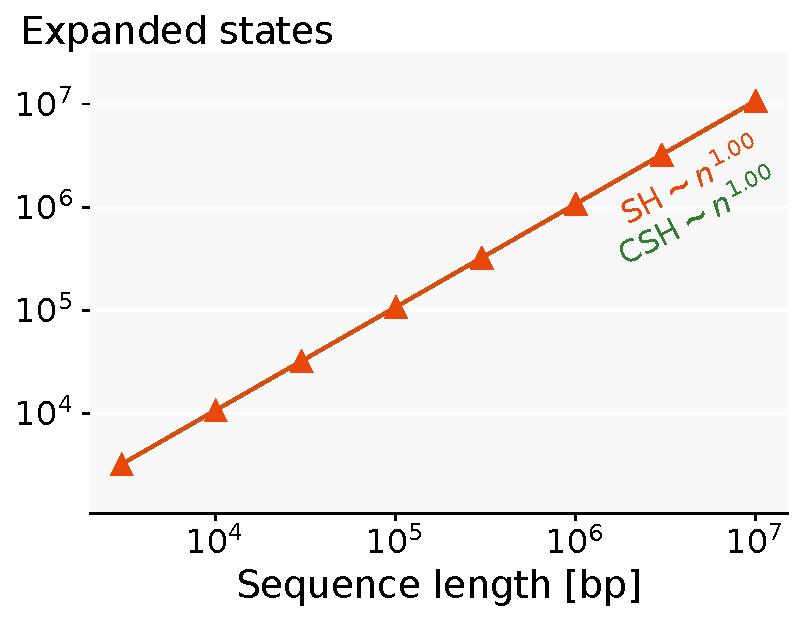
\includegraphics[width=0.24\linewidth]{imgs/fig6/expanded_e0.01_labels.pdf}}
  %\hfill
  \subfloat[$\boldsymbol{e{=}5\%}$, $k{=}15$, $r{=}1$]
  {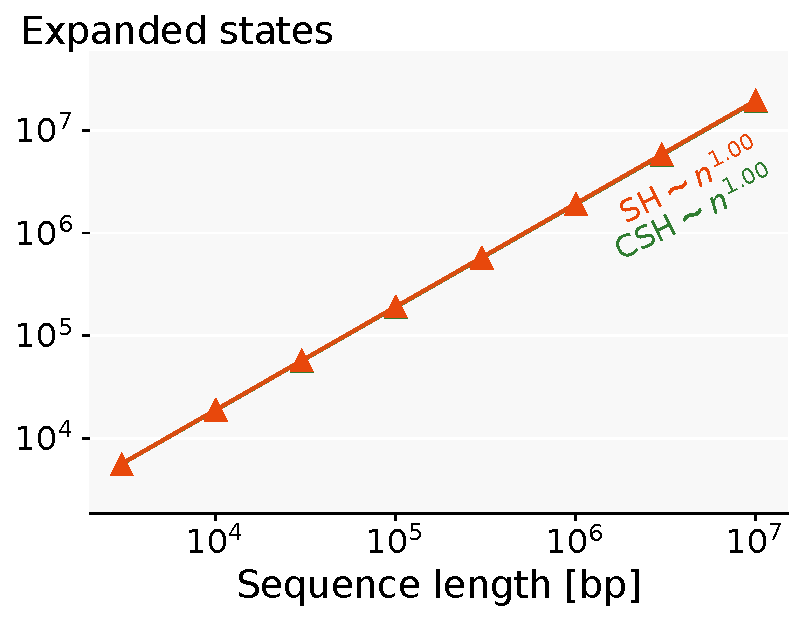
\includegraphics[width=0.48\linewidth]{imgs/fig6/expanded_e0.05_labels.pdf}}
  \hfill
  %\subfloat[$e{=}10\%$, inexact matching]
  %{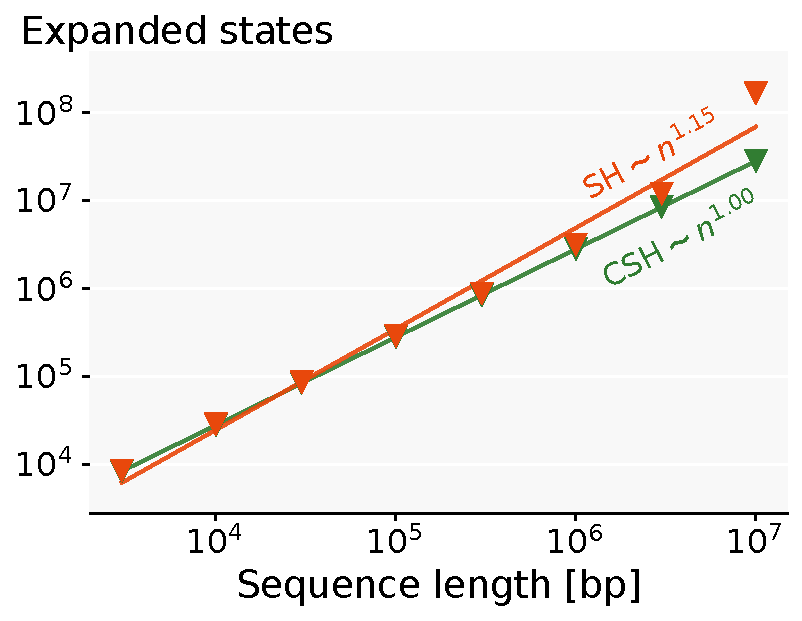
\includegraphics[width=0.24\linewidth]{imgs/fig6/expanded_e0.1_labels.pdf}}
  %\hfill
  \subfloat[$\boldsymbol{e{=}15}\%$, $k{=}15$, $r{=}2$]
  {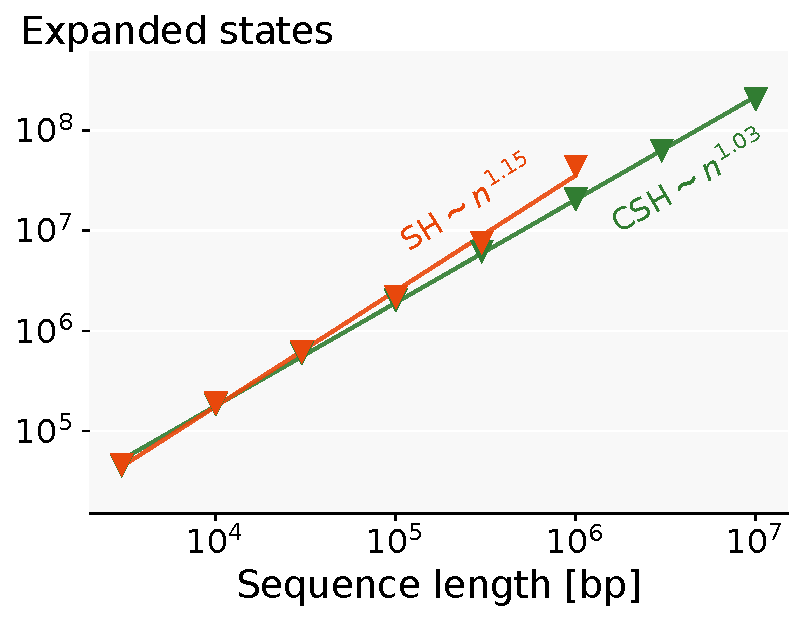
\includegraphics[width=0.48\linewidth]{imgs/fig6/expanded_e0.15_labels.pdf}}
  \caption{Expanded states scaling when aligning \textbf{synthetic sequences},
    corresponding to \cref{GLOBALfig:scaling-n-5,fig:scaling-n-15}.
    }
  %Both heuristics use $k{=}15$ with exact matches
  %($r{=}1$) for $e{\leq} 5\%$ (\shsymbol, \cshsymbol) and inexact matches
  %($r{=}2$) for $e{\ge} 10\%$ (\shsymbolsq, \cshsymbolsq).}
  \label{GLOBALfig:expanded}
\end{figure}
